% Options for packages loaded elsewhere
\PassOptionsToPackage{unicode}{hyperref}
\PassOptionsToPackage{hyphens}{url}
\PassOptionsToPackage{dvipsnames,svgnames,x11names}{xcolor}
%
\documentclass[
  letterpaper,
  DIV=11,
  numbers=noendperiod]{scrartcl}

\usepackage{amsmath,amssymb}
\usepackage{iftex}
\ifPDFTeX
  \usepackage[T1]{fontenc}
  \usepackage[utf8]{inputenc}
  \usepackage{textcomp} % provide euro and other symbols
\else % if luatex or xetex
  \usepackage{unicode-math}
  \defaultfontfeatures{Scale=MatchLowercase}
  \defaultfontfeatures[\rmfamily]{Ligatures=TeX,Scale=1}
\fi
\usepackage{lmodern}
\ifPDFTeX\else  
    % xetex/luatex font selection
\fi
% Use upquote if available, for straight quotes in verbatim environments
\IfFileExists{upquote.sty}{\usepackage{upquote}}{}
\IfFileExists{microtype.sty}{% use microtype if available
  \usepackage[]{microtype}
  \UseMicrotypeSet[protrusion]{basicmath} % disable protrusion for tt fonts
}{}
\makeatletter
\@ifundefined{KOMAClassName}{% if non-KOMA class
  \IfFileExists{parskip.sty}{%
    \usepackage{parskip}
  }{% else
    \setlength{\parindent}{0pt}
    \setlength{\parskip}{6pt plus 2pt minus 1pt}}
}{% if KOMA class
  \KOMAoptions{parskip=half}}
\makeatother
\usepackage{xcolor}
\setlength{\emergencystretch}{3em} % prevent overfull lines
\setcounter{secnumdepth}{3}
% Make \paragraph and \subparagraph free-standing
\makeatletter
\ifx\paragraph\undefined\else
  \let\oldparagraph\paragraph
  \renewcommand{\paragraph}{
    \@ifstar
      \xxxParagraphStar
      \xxxParagraphNoStar
  }
  \newcommand{\xxxParagraphStar}[1]{\oldparagraph*{#1}\mbox{}}
  \newcommand{\xxxParagraphNoStar}[1]{\oldparagraph{#1}\mbox{}}
\fi
\ifx\subparagraph\undefined\else
  \let\oldsubparagraph\subparagraph
  \renewcommand{\subparagraph}{
    \@ifstar
      \xxxSubParagraphStar
      \xxxSubParagraphNoStar
  }
  \newcommand{\xxxSubParagraphStar}[1]{\oldsubparagraph*{#1}\mbox{}}
  \newcommand{\xxxSubParagraphNoStar}[1]{\oldsubparagraph{#1}\mbox{}}
\fi
\makeatother

\usepackage{color}
\usepackage{fancyvrb}
\newcommand{\VerbBar}{|}
\newcommand{\VERB}{\Verb[commandchars=\\\{\}]}
\DefineVerbatimEnvironment{Highlighting}{Verbatim}{commandchars=\\\{\}}
% Add ',fontsize=\small' for more characters per line
\usepackage{framed}
\definecolor{shadecolor}{RGB}{241,243,245}
\newenvironment{Shaded}{\begin{snugshade}}{\end{snugshade}}
\newcommand{\AlertTok}[1]{\textcolor[rgb]{0.68,0.00,0.00}{#1}}
\newcommand{\AnnotationTok}[1]{\textcolor[rgb]{0.37,0.37,0.37}{#1}}
\newcommand{\AttributeTok}[1]{\textcolor[rgb]{0.40,0.45,0.13}{#1}}
\newcommand{\BaseNTok}[1]{\textcolor[rgb]{0.68,0.00,0.00}{#1}}
\newcommand{\BuiltInTok}[1]{\textcolor[rgb]{0.00,0.23,0.31}{#1}}
\newcommand{\CharTok}[1]{\textcolor[rgb]{0.13,0.47,0.30}{#1}}
\newcommand{\CommentTok}[1]{\textcolor[rgb]{0.37,0.37,0.37}{#1}}
\newcommand{\CommentVarTok}[1]{\textcolor[rgb]{0.37,0.37,0.37}{\textit{#1}}}
\newcommand{\ConstantTok}[1]{\textcolor[rgb]{0.56,0.35,0.01}{#1}}
\newcommand{\ControlFlowTok}[1]{\textcolor[rgb]{0.00,0.23,0.31}{\textbf{#1}}}
\newcommand{\DataTypeTok}[1]{\textcolor[rgb]{0.68,0.00,0.00}{#1}}
\newcommand{\DecValTok}[1]{\textcolor[rgb]{0.68,0.00,0.00}{#1}}
\newcommand{\DocumentationTok}[1]{\textcolor[rgb]{0.37,0.37,0.37}{\textit{#1}}}
\newcommand{\ErrorTok}[1]{\textcolor[rgb]{0.68,0.00,0.00}{#1}}
\newcommand{\ExtensionTok}[1]{\textcolor[rgb]{0.00,0.23,0.31}{#1}}
\newcommand{\FloatTok}[1]{\textcolor[rgb]{0.68,0.00,0.00}{#1}}
\newcommand{\FunctionTok}[1]{\textcolor[rgb]{0.28,0.35,0.67}{#1}}
\newcommand{\ImportTok}[1]{\textcolor[rgb]{0.00,0.46,0.62}{#1}}
\newcommand{\InformationTok}[1]{\textcolor[rgb]{0.37,0.37,0.37}{#1}}
\newcommand{\KeywordTok}[1]{\textcolor[rgb]{0.00,0.23,0.31}{\textbf{#1}}}
\newcommand{\NormalTok}[1]{\textcolor[rgb]{0.00,0.23,0.31}{#1}}
\newcommand{\OperatorTok}[1]{\textcolor[rgb]{0.37,0.37,0.37}{#1}}
\newcommand{\OtherTok}[1]{\textcolor[rgb]{0.00,0.23,0.31}{#1}}
\newcommand{\PreprocessorTok}[1]{\textcolor[rgb]{0.68,0.00,0.00}{#1}}
\newcommand{\RegionMarkerTok}[1]{\textcolor[rgb]{0.00,0.23,0.31}{#1}}
\newcommand{\SpecialCharTok}[1]{\textcolor[rgb]{0.37,0.37,0.37}{#1}}
\newcommand{\SpecialStringTok}[1]{\textcolor[rgb]{0.13,0.47,0.30}{#1}}
\newcommand{\StringTok}[1]{\textcolor[rgb]{0.13,0.47,0.30}{#1}}
\newcommand{\VariableTok}[1]{\textcolor[rgb]{0.07,0.07,0.07}{#1}}
\newcommand{\VerbatimStringTok}[1]{\textcolor[rgb]{0.13,0.47,0.30}{#1}}
\newcommand{\WarningTok}[1]{\textcolor[rgb]{0.37,0.37,0.37}{\textit{#1}}}

\providecommand{\tightlist}{%
  \setlength{\itemsep}{0pt}\setlength{\parskip}{0pt}}\usepackage{longtable,booktabs,array}
\usepackage{calc} % for calculating minipage widths
% Correct order of tables after \paragraph or \subparagraph
\usepackage{etoolbox}
\makeatletter
\patchcmd\longtable{\par}{\if@noskipsec\mbox{}\fi\par}{}{}
\makeatother
% Allow footnotes in longtable head/foot
\IfFileExists{footnotehyper.sty}{\usepackage{footnotehyper}}{\usepackage{footnote}}
\makesavenoteenv{longtable}
\usepackage{graphicx}
\makeatletter
\newsavebox\pandoc@box
\newcommand*\pandocbounded[1]{% scales image to fit in text height/width
  \sbox\pandoc@box{#1}%
  \Gscale@div\@tempa{\textheight}{\dimexpr\ht\pandoc@box+\dp\pandoc@box\relax}%
  \Gscale@div\@tempb{\linewidth}{\wd\pandoc@box}%
  \ifdim\@tempb\p@<\@tempa\p@\let\@tempa\@tempb\fi% select the smaller of both
  \ifdim\@tempa\p@<\p@\scalebox{\@tempa}{\usebox\pandoc@box}%
  \else\usebox{\pandoc@box}%
  \fi%
}
% Set default figure placement to htbp
\def\fps@figure{htbp}
\makeatother

\KOMAoption{captions}{tableheading}
\makeatletter
\@ifpackageloaded{caption}{}{\usepackage{caption}}
\AtBeginDocument{%
\ifdefined\contentsname
  \renewcommand*\contentsname{Table of contents}
\else
  \newcommand\contentsname{Table of contents}
\fi
\ifdefined\listfigurename
  \renewcommand*\listfigurename{List of Figures}
\else
  \newcommand\listfigurename{List of Figures}
\fi
\ifdefined\listtablename
  \renewcommand*\listtablename{List of Tables}
\else
  \newcommand\listtablename{List of Tables}
\fi
\ifdefined\figurename
  \renewcommand*\figurename{Figure}
\else
  \newcommand\figurename{Figure}
\fi
\ifdefined\tablename
  \renewcommand*\tablename{Table}
\else
  \newcommand\tablename{Table}
\fi
}
\@ifpackageloaded{float}{}{\usepackage{float}}
\floatstyle{ruled}
\@ifundefined{c@chapter}{\newfloat{codelisting}{h}{lop}}{\newfloat{codelisting}{h}{lop}[chapter]}
\floatname{codelisting}{Listing}
\newcommand*\listoflistings{\listof{codelisting}{List of Listings}}
\makeatother
\makeatletter
\makeatother
\makeatletter
\@ifpackageloaded{caption}{}{\usepackage{caption}}
\@ifpackageloaded{subcaption}{}{\usepackage{subcaption}}
\makeatother

\usepackage{bookmark}

\IfFileExists{xurl.sty}{\usepackage{xurl}}{} % add URL line breaks if available
\urlstyle{same} % disable monospaced font for URLs
\hypersetup{
  pdftitle={简单线性相关和回归},
  pdfauthor={Simonzhou},
  colorlinks=true,
  linkcolor={blue},
  filecolor={Maroon},
  citecolor={Blue},
  urlcolor={Blue},
  pdfcreator={LaTeX via pandoc}}


\title{简单线性相关和回归}
\author{Simonzhou}
\date{2025-02-27}

\begin{document}
\maketitle


\section{简单线性相关和回归}\label{ux7b80ux5355ux7ebfux6027ux76f8ux5173ux548cux56deux5f52}

\subsection{两变量关系分析}\label{ux4e24ux53d8ux91cfux5173ux7cfbux5206ux6790}

\begin{figure}[H]

\pandocbounded{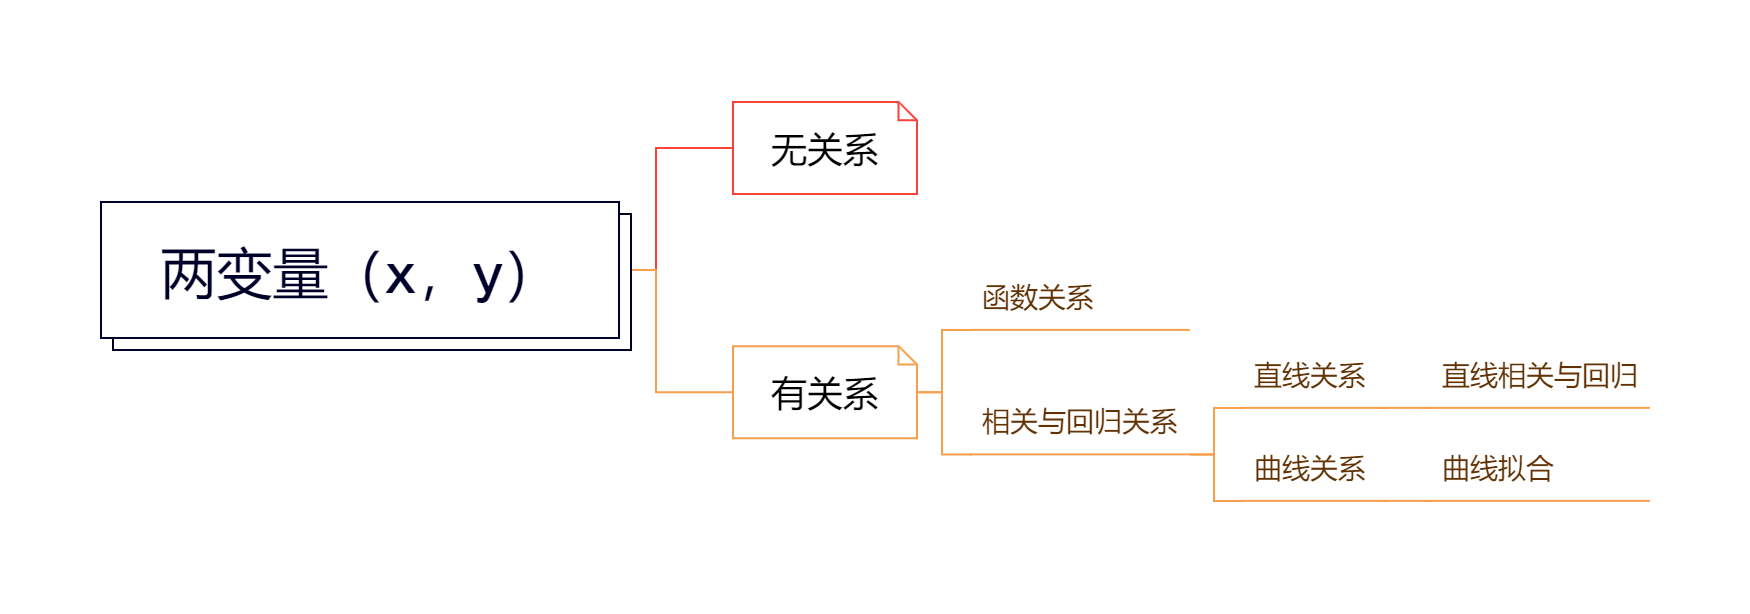
\includegraphics[keepaspectratio]{images/two variables.png}} \hfill{}

\caption{two variables relationship}

\end{figure}%

\subsection{常见相关系数}\label{ux5e38ux89c1ux76f8ux5173ux7cfbux6570}

\subsubsection{直线相关分析基本流程}\label{ux76f4ux7ebfux76f8ux5173ux5206ux6790ux57faux672cux6d41ux7a0b}

\begin{figure}[H]

\pandocbounded{
\includegraphics[keepaspectratio]{images/Draw a scatterplot.png}} \hfill{}

\caption{The basic process of straight-line regression analysis}

\end{figure}%

\subsubsection{三类相关系数总结}\label{ux4e09ux7c7bux76f8ux5173ux7cfbux6570ux603bux7ed3}

\begin{longtable}[]{@{}
  >{\centering\arraybackslash}p{(\linewidth - 2\tabcolsep) * \real{0.3750}}
  >{\raggedright\arraybackslash}p{(\linewidth - 2\tabcolsep) * \real{0.6250}}@{}}
\toprule\noalign{}
\begin{minipage}[b]{\linewidth}\centering
名称
\end{minipage} & \begin{minipage}[b]{\linewidth}\raggedright
适用条件
\end{minipage} \\
\midrule\noalign{}
\endhead
\bottomrule\noalign{}
\endlastfoot
Pearson直线相关系数 &
双变量正态分布的资料\(\rightarrow\)定量\(\rightarrow\)类比t检验、方差分析 \\
列联系数 & 非等级资料\(\rightarrow\)分类\(\rightarrow\)类比卡方检验 \\
Spearman秩相关系数 &
不满足双变量正态分布、分布未知、等级资料\(\rightarrow\)定量+分类\(\rightarrow\)类比秩和检验 \\
\end{longtable}

\subsection{简单直线回归}\label{ux7b80ux5355ux76f4ux7ebfux56deux5f52}

\subsubsection{直线回归分析的基本流程}\label{ux76f4ux7ebfux56deux5f52ux5206ux6790ux7684ux57faux672cux6d41ux7a0b}

\begin{figure}[H]

\pandocbounded{
\includegraphics[keepaspectratio]{images/Draw a scatterplot.png}} \hfill{}

\caption{Draw a scatterplot}

\end{figure}%

\subsubsection{回归方程的建立}\label{ux56deux5f52ux65b9ux7a0bux7684ux5efaux7acb}

选择一组数据集的``最佳拟合直线'',需要设法通过观测数据确定参数\(\alpha\)与\(\beta\)的估计值a和b,使得直线

\[\hat y=a+bx\]

能最佳地反映\((x_i,y_i)\)之间的变化关系,该直线称为一元回归直线。

常用\textbf{最小二乘估计法(least squares
estimation)}来最佳直线,其基本原理是通过最小化残差平方和,使得各观测点到回归直线的纵向距离的平方和最小。

\[
\begin{cases}
a=\bar y-b \bar x\\
b=\frac{\sum\limits_{i=1}^n x_i y_i - \frac{1}{n}(\sum\limits_{i=1}^n x_i)(\sum\limits_{i=1}^n y_i)}{\sum\limits_{i=1}^n x_i^2 - \frac{1}{n}(\sum\limits_{i=1}^n x_i)^2}
\end{cases}
\] 为方便,引入以下记号: \[
SS_{xx}=\sum_{i}(x_i-\bar x)^2=\sum_{i}x_i^2-\frac{1}{n}(\sum_{i}x_i)^2\\
SS_{yy}=\sum_{i}(y_i-\bar y)^2=\sum_{i}y_i^2-\frac{1}{n}(\sum_{i}y_i)^2\\
SS_{xy}=\sum_{i}(x_i-\bar x)(y_i-\bar y)=\sum_{i}x_i y_i-\frac{1}{n}(\sum_{i}x_i)(\sum_{i}y_i)
\]
其中,\(SS_{xx}\)和\(SS_{yy}\)是离均差平方和,\(SS_{xy}\)称为离均差积和。

这样可以简化为: \[
\begin{cases}
a=\bar y-b \bar x\\
b=\frac{SS_{xy}}{SS_{xx}}
\end{cases}
\]

\subsubsection{假设检验}\label{ux5047ux8bbeux68c0ux9a8c}

\begin{enumerate}
\def\labelenumi{\arabic{enumi}.}
\tightlist
\item
  F检验
\end{enumerate}

\(y_i\)的总离均差平方和为:

\[SS_{yy}=\sum_{i}(y_i-\bar y)^2\] 对其做分解,得到等式:

\[SS_{yy}=\sum_{i}^{n}(\hat y_i-\bar y)^2+\sum_{i}^{n}(y_i-\hat y_i)^2\]
\(\sum_{i}^{n}(\hat y_i-\bar y)^2\)为回归平方和(regression sum of
squares),记为\(SS_R\),表示回归估计值\(\hat y_i\)与均数\(\bar y\)的离差平方和,其公式为:

\[
\begin{align}
SS_{yy} &= \sum_{i=1}^{n}(\hat y_i - \bar y)^2 \\
        &= \sum_{i=1}^{n}[a + bx_i - (a + b\bar x)]^2 \\
        &= SS_{xx}b^2 \\
        &= SS_{xy}b
\end{align}
\]
显然,回归平方和\(SS_{R}\)反映的是在y的总变异中由x与y的直线回归关系解释的那部分变异。\(SS_R\)值越大,说明回归直线的拟合效果就越好。

\(\sum_{i}^{n}(y_i-\hat y_i)^2\)为残差平方和(residual sum of
squares),记为\(SS_E\),表示观测值\(y_i\)与回归估计值\(\hat y_i\)的离差平方和,其公式为:
\[SS_E=\sum_{i=1}^{n}(y_i-\hat y_i)^2\]
\(SS_E\)反映了在总变异中扣除自变量x对因变量y的线性影响以后的其他因素(包括x对y的非线性影响和随机误差等)对y变异的影响,也就是在总平方和中无法用y和x线性回归关系解释的部分。\(SS_E\)值越小,说明回归直线的拟合效果就越好。

对公式进行简化: \[\begin{align}
SS_{yy}=&\sum_{i}^{n}(\hat y_i-\bar y)^2+\sum_{i}^{n}(y_i-\hat y_i)^2\\
=&SS_R+SS_E
\end{align}\] 上述三个平方和,各有其相应的自由度\(v\),并有如下关系:
\[v_{yy}=v_R+v_E\\
v_{yy}=n-1,v_R=1,v_E=n-2\]

在\(H_0\)成立的条件下,有:
\[\frac{SS_R}{\sigma^2}\sim \chi^2(v_R),\frac{SS_E}{\sigma^2}\sim \chi^2(v_E)\]
且\(SS_R\)和\(SS_E\)相互独立。

检验统计量:

\[F=\frac{SS_R/v_R}{SS_E/v_E}\]
服从自由度\(v_R=1,v_E=n-2\)的F分布。如果y和x确实存在直线回归关系,那么回归所解释的变异\(SS_R\)应大于其他因素所解释的变异\(SS_E\)。由此可见,F检验正是建立在这个基础上的。

对于给定的检验水准\(\alpha\),
如果\(F>F_{(v_R,v_E),1-\alpha}\),则拒绝\(H_0\),认为直线回归方程有统计学显著性;

如果\(F\leq F_{(v_R,v_E),1-\alpha}\),则不拒绝\(H_0\),尚不能认为直线回归方程有统计学显著性。

\begin{enumerate}
\def\labelenumi{\arabic{enumi}.}
\setcounter{enumi}{1}
\tightlist
\item
  t检验法
\end{enumerate}

\subsection{直线相关与直线回归的比较}\label{ux76f4ux7ebfux76f8ux5173ux4e0eux76f4ux7ebfux56deux5f52ux7684ux6bd4ux8f83}

\begin{longtable}[]{@{}
  >{\centering\arraybackslash}p{(\linewidth - 4\tabcolsep) * \real{0.2055}}
  >{\centering\arraybackslash}p{(\linewidth - 4\tabcolsep) * \real{0.2055}}
  >{\raggedright\arraybackslash}p{(\linewidth - 4\tabcolsep) * \real{0.5890}}@{}}
\toprule\noalign{}
\begin{minipage}[b]{\linewidth}\centering
区别与联系
\end{minipage} & \begin{minipage}[b]{\linewidth}\centering
类目
\end{minipage} & \begin{minipage}[b]{\linewidth}\raggedright
内容
\end{minipage} \\
\midrule\noalign{}
\endhead
\bottomrule\noalign{}
\endlastfoot
区别 & 资料要求 & 1.
线性相关要求X,Y服从双变量正态分布,对这种资料进行回归分析称为\(\textrm{II}\)型回归,即可以把X当自变量,也可以当因变量,反之亦然。2.
线性回归要求Y在给定X值时服从正态分布,X可以是精确测量和严格控制的变量,这时的回归称为\textrm{I}型回归,即不可以把X当因变量,Y当自变量进行回归分析。 \\
& 应用 & 1.
线性相关用来表达两个变量间的互依关系,两个变量的研究地位是相等的,谁做X,谁做Y都可以;2.
线性回归用来表达两个变量间的依存变化的数量关系,即一个变量(为因变量Y)如何依存于另一个变量(为自变量X)而变化,两个变量的研究地位是不相等的。 \\
& 意义 & 1.
相关系数r说明具有线性关系的两个变量之间的密切程度和相关方向;2.
回归系数b表示X每变化一个单位所导致的Y的平均变化量。 \\
& r和b的取值范围 &
r没有单位,而b有单位(其单位是:Y的单位/X的单位),所以导致两者的取值范围不同;
\(-1 \le r \le 1\),\(-\infty<b<+\infty\) \\
& r和b的计算公式不同 &
\(r=\frac{l_{xy}}{\sqrt{l_{xx}l_{yy}}}\),\(b=\frac{l_{xy}}{l_{xx}}\) \\
联系 & 符号 &
对于既可以做相关又可作回归的同一组资料,计算出r与b的正负号相同 \\
& 假设检验 &
对于同一组资料,相关系数和回归系数的假设检验等价。即有:\(t_b=t_r\) \\
& 相互换算 &
对于同一组资料,相关系数和回归系数可通过下式换算:\(b=r\frac{S_Y}{S_X}\),式中的\(S_X,S_Y\)分别是\(X,Y\)的标准差 \\
& 用回归解释相关 &
又决定系数\(R^2=\frac{SS_{回}}{SS_{总}}\),当总平方和的大小决定了相关的密切程度,回归平方和越接近总平方和,则\(R^2\)越接近1,相关的效果越好,说明回归效果越好,相关的密切程度也越高。 \\
\end{longtable}

\textbf{notice}:关于双变量正态分布

双元正态变量是指两个随机变量同时遵循正态分布的情况,通常记作
\((X, Y) \sim N(\mu, \Sigma)\),其中 \(\mu\) 是均值向量,\(\Sigma\)
是协方差矩阵。

数学定义

\begin{verbatim}
1.  均值向量:对于双元正态变量 $(X, Y)$,均值向量为:
\end{verbatim}

\[\mu = \begin{pmatrix}
\mu_X \\
\mu_Y
\end{pmatrix}\]

其中 \(\mu_X\) 和 \(\mu_Y\) 分别是随机变量 \(X\) 和 \(Y\) 的均值。 2.
协方差矩阵:协方差矩阵为:

\[\Sigma = \begin{pmatrix}
\sigma_X^2 & \sigma_{XY} \\
\sigma_{XY} & \sigma_Y^2
\end{pmatrix}\]

其中 \(\sigma_X^2\) 和 \(\sigma_Y^2\) 是 \(X\) 和 \(Y\)
的方差,\(\sigma_{XY}\) 是它们之间的协方差。

性质

\begin{verbatim}
•   边缘分布:$X$ 和 $Y$ 的边缘分布也是正态分布。
•   条件分布:给定 $X$ 的值,$Y$ 的条件分布也是正态分布。
•   相关性:协方差矩阵的值可以用来判断 X 和 Y 之间的相关性。如果 $\sigma_{XY} > 0$,则两者正相关;如果 $\sigma_{XY} < 0$,则负相关。
\end{verbatim}

示例

假设有一组数据描述学生的身高 \(X\) 和体重 \(Y\),并且假设 \((X, Y)\)
服从双元正态分布:

\begin{verbatim}
•   均值向量:
\end{verbatim}

\[\mu = \begin{pmatrix}
170 \\
65
\end{pmatrix}\]

表示身高的均值为 170 厘米,体重的均值为 65 千克。 • 协方差矩阵:

\[\Sigma = \begin{pmatrix}
100 & 20 \\
20 & 25
\end{pmatrix}\]

这里,身高的方差为 100,体重的方差为 25,协方差为
20,表示身高和体重之间存在正相关关系。

在这个示例中,如果我们知道某个学生的身高为 180
厘米,我们可以利用条件分布来预测他的体重,这个体重的预测值也是正态分布。

我们用一个图形来展示:

\begin{Shaded}
\begin{Highlighting}[]
\DocumentationTok{\#\# 安装和加载所需的包}
\CommentTok{\#install.packages("plotly")}
\CommentTok{\#install.packages("mvtnorm")}
\FunctionTok{library}\NormalTok{(plotly)}
\FunctionTok{library}\NormalTok{(mvtnorm)}
\FunctionTok{library}\NormalTok{(webshot2)}

\CommentTok{\# 创建网格数据}
\NormalTok{x }\OtherTok{\textless{}{-}} \FunctionTok{seq}\NormalTok{(}\DecValTok{150}\NormalTok{, }\DecValTok{190}\NormalTok{, }\AttributeTok{length.out =} \DecValTok{100}\NormalTok{)}
\CommentTok{\#身高150{-}190,等距的100个值}
\NormalTok{y }\OtherTok{\textless{}{-}} \FunctionTok{seq}\NormalTok{(}\DecValTok{50}\NormalTok{, }\DecValTok{80}\NormalTok{, }\AttributeTok{length.out =} \DecValTok{100}\NormalTok{)}
\CommentTok{\#体重50{-}80,等距的100个值}
\NormalTok{grid }\OtherTok{\textless{}{-}} \FunctionTok{expand.grid}\NormalTok{(}\AttributeTok{X =}\NormalTok{ x, }\AttributeTok{Y =}\NormalTok{ y)}
\CommentTok{\#生成 x 和 y 的所有组合,用于构建一个网格数据框,以便计算多元正态分布的概率密度。}

\CommentTok{\# 设置均值和协方差矩阵}
\NormalTok{mu }\OtherTok{\textless{}{-}} \FunctionTok{c}\NormalTok{(}\DecValTok{170}\NormalTok{, }\DecValTok{65}\NormalTok{)}
\CommentTok{\#设置双元正态分布的均值向量,表示均值分别为身高 170 cm 和体重 65 kg}

\NormalTok{sigma }\OtherTok{\textless{}{-}} \FunctionTok{matrix}\NormalTok{(}\FunctionTok{c}\NormalTok{(}\DecValTok{100}\NormalTok{, }\DecValTok{20}\NormalTok{, }\DecValTok{20}\NormalTok{, }\DecValTok{25}\NormalTok{), }\AttributeTok{nrow =} \DecValTok{2}\NormalTok{)}
\CommentTok{\#设置协方差矩阵,表示身高的方差为 100,体重的方差为 25,身高和体重之间的协方差为 20}

\CommentTok{\# 计算概率密度}
\NormalTok{z }\OtherTok{\textless{}{-}} \FunctionTok{dmvnorm}\NormalTok{(}\FunctionTok{as.matrix}\NormalTok{(grid), }\AttributeTok{mean =}\NormalTok{ mu, }\AttributeTok{sigma =}\NormalTok{ sigma)}
\CommentTok{\#计算每个网格点上双元正态分布的概率密度。}

\CommentTok{\# 将概率密度矩阵转换为适合绘图的形状}
\NormalTok{z\_matrix }\OtherTok{\textless{}{-}} \FunctionTok{matrix}\NormalTok{(z, }\AttributeTok{nrow =} \DecValTok{100}\NormalTok{, }\AttributeTok{ncol =} \DecValTok{100}\NormalTok{)}

\CommentTok{\# 绘制三维表面图}
\FunctionTok{plot\_ly}\NormalTok{(}\AttributeTok{x =}\NormalTok{ x, }\AttributeTok{y =}\NormalTok{ y, }\AttributeTok{z =}\NormalTok{ z\_matrix, }\AttributeTok{type =} \StringTok{"surface"}\NormalTok{) }\SpecialCharTok{\%\textgreater{}\%}
  \FunctionTok{layout}\NormalTok{(}\AttributeTok{title =} \FunctionTok{list}\NormalTok{(}\AttributeTok{text =} \StringTok{"双元正态分布的三维概率密度图"}\NormalTok{, }\AttributeTok{y=}\FloatTok{0.95}\NormalTok{),}
         \AttributeTok{scene =} \FunctionTok{list}\NormalTok{(}\AttributeTok{xaxis =} \FunctionTok{list}\NormalTok{(}\AttributeTok{title =} \StringTok{"身高 (cm)"}\NormalTok{),}
                      \AttributeTok{yaxis =} \FunctionTok{list}\NormalTok{(}\AttributeTok{title =} \StringTok{"体重 (kg)"}\NormalTok{),}
                      \AttributeTok{zaxis =} \FunctionTok{list}\NormalTok{(}\AttributeTok{title =} \StringTok{"概率密度"}\NormalTok{)))}
\end{Highlighting}
\end{Shaded}

\begin{figure}[H]

\pandocbounded{
\includegraphics[keepaspectratio]{10-regression-correlation_files/figure-pdf/unnamed-chunk-1-1.pdf}} \hfill{}

\caption{Binary normal distribution}

\end{figure}%

注:上述图像在被转换为PDF文件时,会发生报错:Quarto 文档中包含了一些生成
HTML 输出的函数(比如交互式图表或其他 HTML
小部件),但你当前的目标输出格式是 PDF。由于 PDF
是静态格式,无法直接渲染 HTML 内容,Quarto 会报错并停止执行。

解决方案,此章节不转换为PDF格式,或者:

如果你仍想输出 PDF,但希望将 HTML 小部件作为静态截图嵌入,可以安装 R 的
webshot 或 webshot2 包。Quarto 会利用它们将 HTML 内容转换为图片。

需要安装:

\begin{Shaded}
\begin{Highlighting}[]
\FunctionTok{install.packages}\NormalTok{(}\StringTok{"webshot2"}\NormalTok{)}
\end{Highlighting}
\end{Shaded}

然后在这段程序的前部导入该包:\texttt{library(webshot2)}。




\end{document}
